%%%%%%%%%%%%%%%%%%%%%%%%%%%%%%%%%%%%%%%%%%%%%%%%%%%%%%%%%%%%%%%%%%%%%%%
%
%   Presentation of Beamer UNL Theme
%   Beamer Presentation by Chris Bourke
%
%%%%%%%%%%%%%%%%%%%%%%%%%%%%%%%%%%%%%%%%%%%%%%%%%%%%%%%%%%%%%%%%%%%%%%%

\documentclass{beamer}

\usetheme[hideothersubsections]{UNLTheme}
\usepackage[postscript]{ucs}
\usepackage[utf8x]{inputenc}
\usepackage{amsmath}
\usepackage{amssymb}
\usepackage{amsthm}
\usepackage{mathtools}
\title{Performance Modeling and
Design of Computer Systems- Ch 12 \\
Transition to Continuous-Time
Markov Chains}
\author{Debobroto Das Robin} %
\institute{Kent State University}
\date{Spring 2020}




\begin{document}

%{% open a Local TeX Group
%\setbeamertemplate{sidebar}{}
\begin{frame}
        \titlepage
        \begin{center}
    \href{mailto:drobin@kent.edu}{\color{blue}{\texttt{drobin@kent.edu}}}
        \end{center}
\end{frame}

\begin{frame}
\frametitle{Overview} % Table of contents slide, comment this block out to remove it
\tableofcontents % Throughout your presentation, if you choose to use \section{} and \subsection{} commands, these will automatically be printed on this slide as an overview of your presentation
\end{frame}



\section{ Continuous-Time Markov Chain (CTMC) }



\begin{frame} 
\frametitle{Continuous-Time Markov Chain (CTMC) }
\framesubtitle{\textbf{\textit{Definition}}}
\begin{itemize}
\item  \textbf{Continuous-Time Markov Chain (CTMC)}:  a continuous-time
stochastic process $\{X(t), t \geq 0\}$ s.t., $ \forall s, t \geq 0$ and $ \forall i, j, x(u)$,
$$P \{X(t + s) = j | X(s) = i, X(u) = x(u), 0 \leq u \leq s\}  $$
$$= P \{X(t + s) = j | X(s) = i\} (by M.P.) $$
$$ = P \{X(t) = j | X(0) = i\} = P_{ij} (t) (stationarity)$$
\item We assume throughout that the state space is countable (though continuous)
\item  $\tau_i =$ time until the CTMC leaves state $i$, given that it is currently in state i. 
\item $\tau_i $ is memoryless and exponentially distributed

\end{itemize}


	
\end{frame}



\begin{frame} 
\frametitle{Continuous-Time Markov Chain (CTMC)-2 }
\framesubtitle{\textbf{\textit{Explanation}}}
\begin{itemize}

\item A CTMC 
\begin{itemize}
\item The amount of time the process spends in state $i$ before making a transition is
Exponentially distributed with some rate ( $v_i$ ).
\item  When the process leaves state $i$, it will next enter state $j$ with probability
($p_{ij}$ ) independent of the time spent at state $i$.
\end{itemize}

\item $p_{ij}$ ,  probability of  when we leave $i$ we next go to state $j$ , is and independent of time, $t$, (by stationarity property). 
\item $p_{ij}$ is independent of the time spent in state $i$, $\tau_i$ ( by the Markovian property).
\begin{figure}
        \begin{center}
		\includegraphics[scale=0.5]{images/ctmc.jpeg}
        \end{center}
		\end{figure}

\end{itemize}
	
\end{frame}

\begin{frame} 
\frametitle{Continuous-Time Markov Chain (CTMC) }
\framesubtitle{\textbf{\textit{Example}}}
\begin{itemize}

\item Suppose we are in state $i$, where $i \geq 1$. Then the next event is either an arrival or a departure.

\begin{figure}
        \begin{center}
		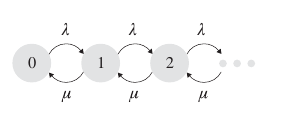
\includegraphics[scale=0.5]{images/single_server_network.jpeg}
        \end{center}
		\end{figure}
\item $X_A = $ time to next arraival.  $X_A\sim  Exp(\lambda)$ regardless of
how long we are in the current state. 
\item $X_D$ = time to the
next departure. Then $X_D \sim Exp(\mu)$ regardless of how long we are in
current state. $X_A$ \& $X_D$ are independent of each other.
\item Arrival \& departure events happen in parallel. One of these, will occur first. So, $\tau_i$ = ime until we leave state $i$, has the
distribution: $\tau_i \sim Exp(\lambda + \mu) \rightarrow v_i = \lambda + \mu)$
\item probability of when we leave state i we will next go to state $(i + 1)$ is
$P \{X_A < X_D \} = \frac{\lambda}{\lambda + \mu}$


\end{itemize}

\end{frame}


\section { Solving CTMCs}


\begin{frame} 
\frametitle{Solving CTMCs-1 }
\framesubtitle{\textbf{\textit{}}}
\begin{itemize}
\item \textbf{Goal:} Finding $\tau_j = \lim_{t \rightarrow \infty} P_{ij} (t) =$ limiting probability of being in state j
\item \textbf{Solution:} Model CTMC as DTMC and find solution
\item We are not discussing full details of derivation
\item \textbf{Balance Equation:}  the rate at which jobs leave state $j$ in the CTMC =  the rate at which jobs enter state j in the CTMC, for each state j .
$$\: \pi_j v_j = \sum_i \pi_i Q_{ij} $$
\item  \textbf{LHS}=total rate of transitions leaving state j= limiting probability of being in state j($\pi_j) $ * rate the MC leaves state j given that it is in state $j (v_j))$ .


\end{itemize}

\end{frame}


\begin{frame} 
\frametitle{Solving CTMCs -2}
\framesubtitle{\textbf{\textit{}}}
\begin{itemize}

\item \textbf{RHS}= total rate
of transitions entering state j from any state= $\sum \forall i $ (limiting proba-
bility of being in state $i (\pi_i)$ *   rate the MC leaves state $i$ to go to state $j$ given that it is in state $i \: ( q_{ij})$  

\item Balance Equation Become
$$ \Rightarrow \: \pi_j \sum_i \pi_i Q_{ij} = \sum_i \pi_i Q_{ij} $$

\item Just solve the balance equation to find the limiting probability
\end{itemize}

\end{frame}

\section{Appllicability of DTMC results}

\begin{frame} 
\frametitle{ Summary Theorem for CTMCs}
\framesubtitle{\textbf{\textit{}}}
\begin{itemize}

\item  CTMCs can basically be viewed as DTMCs in which the time step goes to
zero ($t \rightarrow 0$),  
$\Rightarrow $  all the ergodicity theory that we developed for DTMCs carries over to CTMCs.

\item \textbf{Summary Theorem for CTMCs:} Given an irreducible CTMC,
suppose $ \exists \pi_i $ s.t. $\forall j$ ,
$$\pi_j v_j = \sum_i \pi_i q_{ij}$$ and 
$$\sum_i \pi_i = 1$$

\item \textit{In an irreducible Markov Chain, the process can go from any state to any state, whatever be the number of steps it requires.}

\end{itemize}
\end{frame}





\end{document}